\documentclass[times,t]{beamer}
\usepackage{amssymb}
\usepackage{amsmath}
\usepackage{amsfonts}
\usepackage{lmodern} 
\input{sym.tex}
\setbeamertemplate{navigation symbols}{}

\title{ECE 417/598: Eigen Value Decomposition, Singular Value Decompsition }
\author{Vikas Dhiman.  }
\date{March 4, 2022}
\begin{document}
\newcommand{\ubfu}{\underline{\bfu}}
\begin{frame}
  \includegraphics[width=\linewidth]{media/lane-from-points.pdf}
  \begin{align*}
    \ubfu_1 &= [100, 98, 1]^\top\\
    \ubfu_2 &= [105, 95, 1]^\top\\
    \ubfu_3 &= [107, 90, 1]^\top\\
    \ubfu_4 &= [110, 85, 1]^\top
    \end{align*}
    Find  the line $\bfl$ such that it is the ``closest line'' passing through
    $\bfu_1, \dots, \bfu_4$.
\end{frame}

\begin{frame}
  \[
  U = \begin{bmatrix}\bfu_1^\top  \\
    \bfu_2^\top \\
    \bfu_3^\top \\
    \bfu_4^\top
  \end{bmatrix}
  \]
  We want to solve for $\bfl$ such that
  \[
    U \bfl = 0
  \]
\end{frame}


\begin{frame}{Eigenvalues  and Eigenvectors}

For a  square  matrix $A$, the $\lambda_i$ and  $\bfx_i$ that satisfy  the
following equation are called eigenvalues and  eigenvectors  respectively.
\begin{align}
  A  \bfx &= \lambda \bfx \text{ or } (A  - \lambda I)\bfx  = 0
\end{align}

$\lambda$ is   chosen to ensure  that   $A  -  \lambda I$  has null space,
hence, characteristic   equation
\begin{align}
  \det(A  - \lambda I) = 0 
 \end{align}

 For  symmetrix matrix $A =  A^\top$, eigenvalues  are  real, and eigenvectors
 are orthonormal,
 \begin{align}
   &A[\bfx_1, \dots,   \bfx_n]  = [\bfx_1, \dots,   \bfx_n]\begin{bmatrix}\lambda_1 &   \dots   &  0 \\
     \vdots   &   \ddots &  \vdots \\
   0 &   \dots  &  \lambda_n \end{bmatrix}
                  \\
   &A  S = S  \Lambda
   \\
   &\text{  if   }  A =  A^\top \text{ then   }  A   = S \Lambda S^\top
   \end{align}


\end{frame}


\begin{frame}{Numerical example}
  \[
  A   =  \begin{bmatrix}
    1 &   2  &  3  \\
    4 & 5 &   6 \\
    2 & 4 &   6
  \end{bmatrix}
  \]
Find eigen values and eigen vectors.
\end{frame}


\begin{frame}{Singular Value  Decomposition (SVD)}
  \begin{align}
    A  &=   U  \begin{bmatrix}\Sigma   &  0  \\   0  &  0 \end{bmatrix} V^\top \\
    A^\top A &= V \Sigma^2  V^{-1} \\
    A^\top A \bfv_i  &= \lambda_i \bfv_i & \lambda_i = \sigma_i^2\\
    A V   &= U \begin{bmatrix}\Sigma   &  0  \\   0  &  0 \end{bmatrix}\\
    U^+   &=  \Sigma^{-1}AV^+
    \end{align}
\end{frame}

\begin{frame}{Numerical example}
  Find singular value decomposition
  \[
    A   =  \begin{bmatrix}
      1 &   2  &  3  \\
      4 & 5 &   6 \\
      2 & 4 &   6
    \end{bmatrix}
  \]
\end{frame}


  \includegraphics[width=\linewidth]{media/homography-maps-a-line-to-a-line.png}
\end{frame}
\begin{frame}{Examples  of  Homography}
  \includegraphics[width=\linewidth]{media/examples-of-homography.png}
\end{frame}

\begin{frame}
  \includegraphics[width=0.60\linewidth]{media/audi top view camera.jpg}
\end{frame}

\begin{frame}{Computing Homography}
  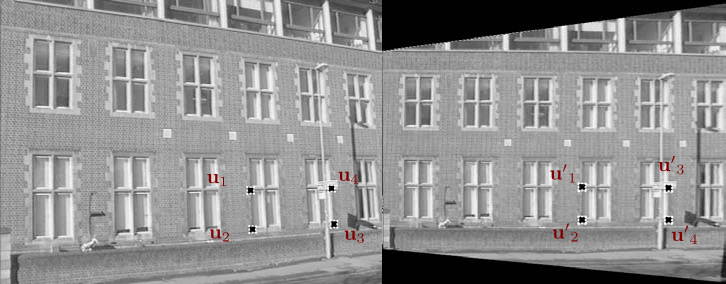
\includegraphics[width=0.45\linewidth]{media/removing-perspective-distortion.png}
  \includegraphics[width=0.45\linewidth]{media/removing-perspective-distortion-b.png}
\end{frame}


\begin{frame}{Computing Homography}
  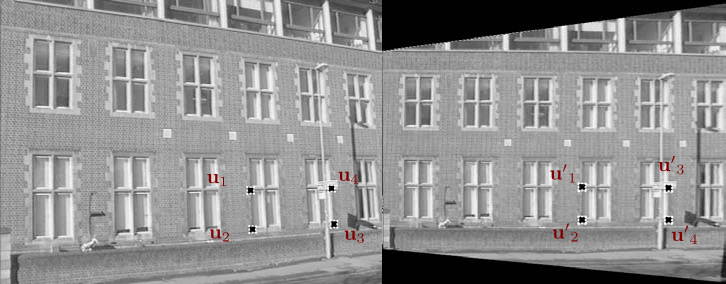
\includegraphics[width=0.45\linewidth]{media/removing-perspective-distortion.png}
  \includegraphics[width=0.45\linewidth]{media/removing-perspective-distortion-b.png}
\end{frame}

\begin{frame}{Solving for Homography derivation}
\end{frame}

\begin{frame}{Direct Linear Transformation   (DLT) algorithm}
  \includegraphics[width=\linewidth]{media/DLT-algorithm.png}
\end{frame}

\begin{frame}{2D homography}
  Given a set of points $\bfx_i \in \bbP^2$ and a corresponding set of
  points $\bfx'_i \in \bbP^2$, compute the projective transformation that takes each
  $\bfx_i$ to $\bfx'_i$ . In a practical situation, the points $\bfx_i$ and   $\bfx'_i$  are points in two images
  (or the same image), each image being considered as a projective plane  $\bbP^2$.
\end{frame}

\begin{frame}{3D  to  2D camera projection matrix estimation}
  Given a set of points $\bfX_i$ in 3D space, and a set
  of corresponding points $\bfx_i$ in an image, find the 3D to 2D projective
  $\bfP$ mapping
  that maps $\bfX_i$ to $\bfx_i  =  \bfP\bfX_i$.
\end{frame}

\end{document}